% PRD flow chart 2: two ways of putting the SS source on the contour.
\documentclass[tikz,border=2pt]{standalone}
\usepackage[T1]{fontenc}
\usepackage{lmodern}
\usepackage{amsmath,amssymb}
\usetikzlibrary{arrows.meta,positioning,calc}
\newcommand{\PP}{\Phi^{\rm P}}
\begin{document}
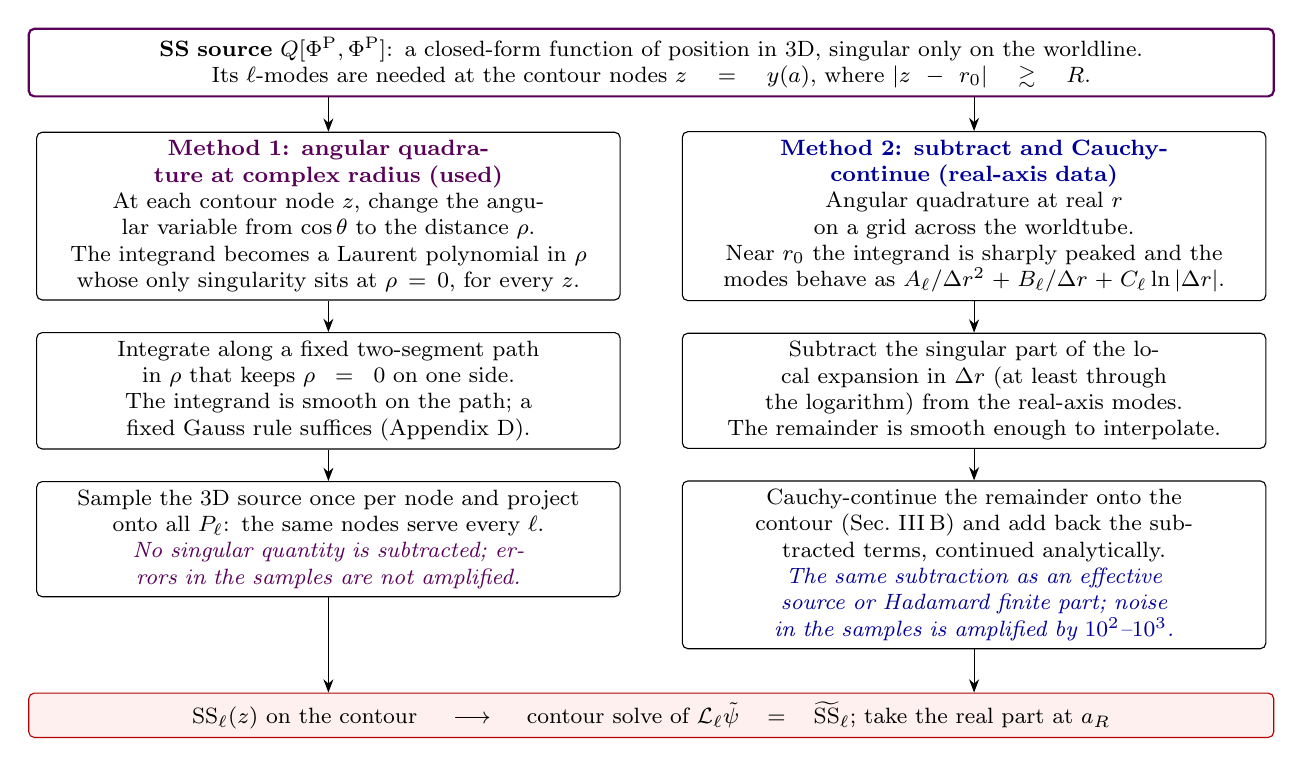
\begin{tikzpicture}[>=Stealth, font=\footnotesize,
  box/.style={draw, rounded corners=2pt, align=center, inner sep=3pt, text width=#1, fill=white},
  head/.style={font=\footnotesize\bfseries, align=center, text width=7.2cm}]
\node[box=15.6cm, draw=violet!70!black, thick] (top) at (0,0)
  {\textbf{SS source} $Q[\PP,\PP]$: a closed-form function of position in 3D, singular only on the worldline.\\
   Its $\ell$-modes are needed at the contour nodes $z=y(a)$, where $|z-r_0|\gtrsim R$.};
% left column: complex-r quadrature
\node[box=7.2cm] (l1) at (-4.1,-1.95)
  {\textcolor{violet!70!black}{\textbf{Method 1: angular quadrature at complex radius (used)}}\\At each contour node $z$, change the angular variable from $\cos\theta$ to the distance $\rho$.\\
   The integrand becomes a Laurent polynomial in $\rho$ whose only singularity sits at $\rho=0$, for every $z$.};
\node[box=7.2cm] (l2) [below=0.40cm of l1]
  {Integrate along a fixed two-segment path in $\rho$ that keeps $\rho=0$ on one side.\\
   The integrand is smooth on the path; a fixed Gauss rule suffices (Appendix~D).};
\node[box=7.2cm] (l3) [below=0.40cm of l2]
  {Sample the 3D source once per node and project onto all $P_\ell$: the same nodes serve every $\ell$.\\
   \textit{\textcolor{violet!70!black}{No singular quantity is subtracted; errors in the samples are not amplified.}}};
% right column: subtraction + Cauchy
\node[box=7.2cm] (r1) at (4.1,-1.95)
  {\textcolor{blue!60!black}{\textbf{Method 2: subtract and Cauchy-continue (real-axis data)}}\\Angular quadrature at real $r$ on a grid across the worldtube.\\
   Near $r_0$ the integrand is sharply peaked and the modes behave as $A_\ell/\Delta r^2+B_\ell/\Delta r+C_\ell\ln|\Delta r|$.};
\node[box=7.2cm] (r2) [below=0.40cm of r1]
  {Subtract the singular part of the local expansion in $\Delta r$ (at least through the logarithm) from the real-axis modes.\\
   The remainder is smooth enough to interpolate.};
\node[box=7.2cm] (r3) [below=0.40cm of r2]
  {Cauchy-continue the remainder onto the contour (Sec.~III\,B) and add back the subtracted terms, continued analytically.\\
   \textit{\textcolor{blue!60!black}{The same subtraction as an effective source or Hadamard finite part; noise in the samples is amplified by $10^2$--$10^3$.}}};
\path let \p1=(l3.south), \p2=(r3.south) in coordinate (lowest) at (0,{min(\y1,\y2)});
\node[box=15.6cm, draw=red!70!black, fill=red!6] (bot) [below=0.55cm of lowest]
  {$\mathrm{SS}_\ell(z)$ on the contour $\;\longrightarrow\;$ contour solve of $\mathcal L_\ell\tilde\psi=\widetilde{\mathrm{SS}}_\ell$; take the real part at $a_R$};
\draw[->] (top.south -| l1) -- (l1.north);
\draw[->] (top.south -| r1) -- (r1.north);
\draw[->] (l1) -- (l2); \draw[->] (l2) -- (l3);
\draw[->] (r1) -- (r2); \draw[->] (r2) -- (r3);
\draw[->] (l3.south) -- (l3.south |- bot.north);
\draw[->] (r3.south) -- (r3.south |- bot.north);
\end{tikzpicture}
\end{document}
